\documentclass[]{article}
\usepackage{listings}
\usepackage[MeX]{polski}
\usepackage[utf8]{inputenc}
\usepackage{graphicx}
\usepackage{xcolor}
\usepackage{float}
\usepackage{ulem}
\usepackage{placeins}
\usepackage{listings}
\usepackage{geometry}
\newgeometry{lmargin=3cm, rmargin=3cm}

\usepackage{trace}
\title{TECY - Projekt 3}
\author{Małgorzata Pszczółkowska - 311423\\ Anastasiya Ronskaya - 317058 \\ Konrad Kotlicki - 310958 \\Sebastian Skrzek - 311442}
\begin{document}
\maketitle
\tableofcontents
\section{Wskaźnik}
Nasz wskaźnik do danych to:
$3+8+8+2=2\textbf{\underline{1}}$
\begin{figure}[H]
	\centering
	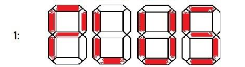
\includegraphics[width=0.57\textwidth]{plus.png}
	\caption{Nasz wzór do realizacji}
\end{figure}
\section{Stany}
\begin{figure}[H]
	\centering
	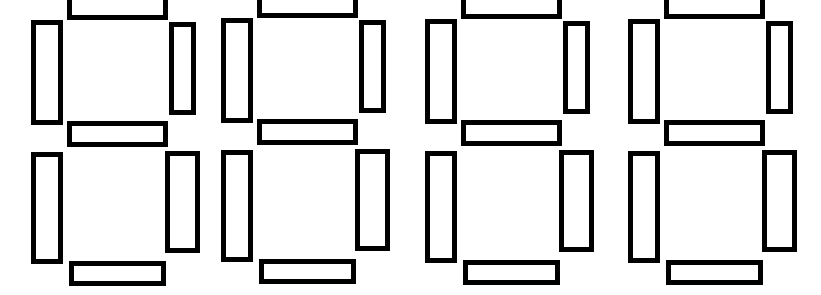
\includegraphics[width=0.57\textwidth]{stan0.png}
	\caption{Widok stanu 0.}
\end{figure}
\begin{figure}[H]
	\centering
	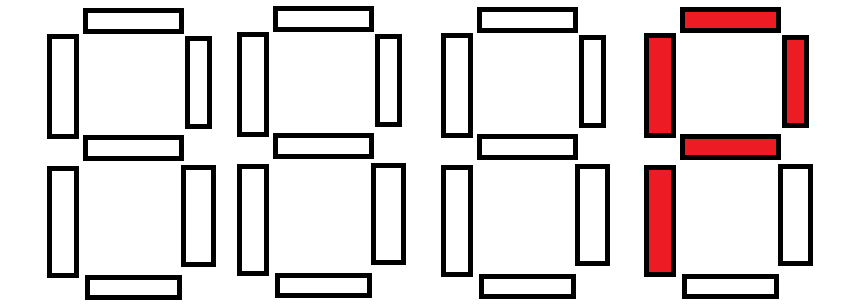
\includegraphics[width=0.57\textwidth]{stan1.png}
	\caption{Widok stanu 1.}
\end{figure}
\begin{figure}[H]
	\centering
	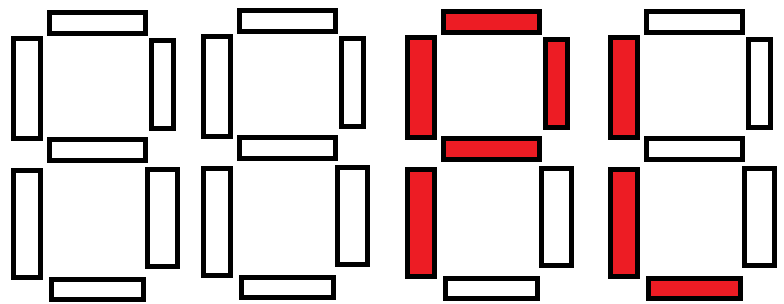
\includegraphics[width=0.57\textwidth]{stan2.png}
	\caption{Widok stanu 2.}
\end{figure}
\begin{figure}[H]
	\centering
	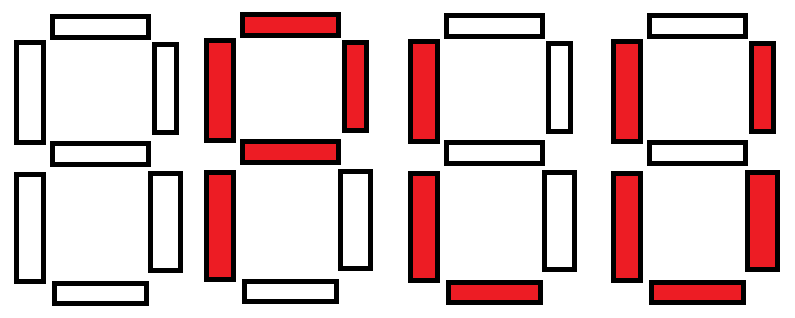
\includegraphics[width=0.57\textwidth]{stan3.png}
	\caption{Widok stanu 3.}
\end{figure}
\begin{figure}[H]
	\centering
	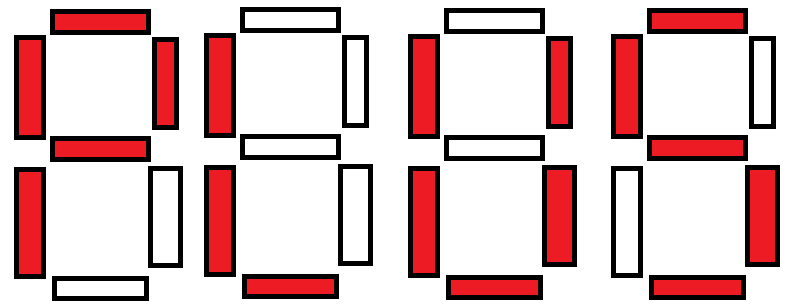
\includegraphics[width=0.57\textwidth]{stan4.png}
	\caption{Widok stanu 4.}
\end{figure}
\begin{figure}[H]
	\centering
	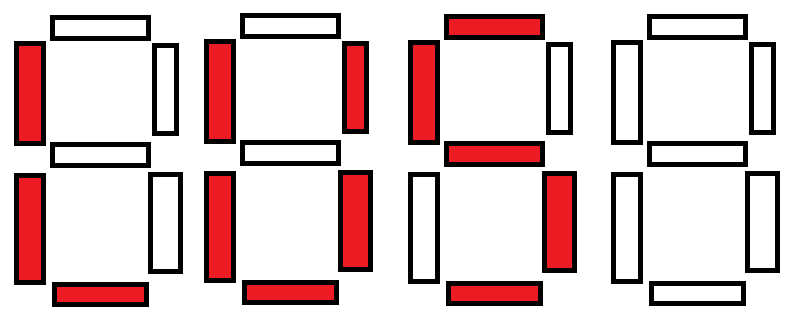
\includegraphics[width=0.57\textwidth]{stan5.png}
	\caption{Widok stanu 5.}
\end{figure}
\begin{figure}[H]
	\centering
	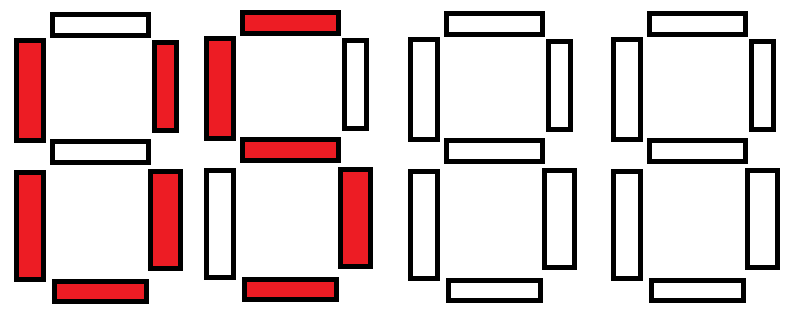
\includegraphics[width=0.57\textwidth]{stan6.png}
	\caption{Widok stanu 6.}
\end{figure}
\begin{figure}[H]
	\centering
	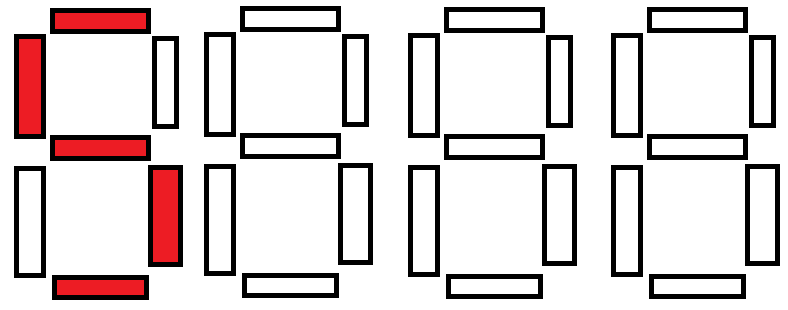
\includegraphics[width=0.57\textwidth]{stan7.png}
	\caption{Widok stanu 7.}
\end{figure}
\newpage
\section{Funkcja stanu następnego}
Na początku narysujemy schemat działania funkcji. Zmienna x decyduje o kierunku animacji liter (dla x=1 od lewej do prawej, a dla x=0 od prawej do lewej).
\begin{figure}[H]
	\centering
	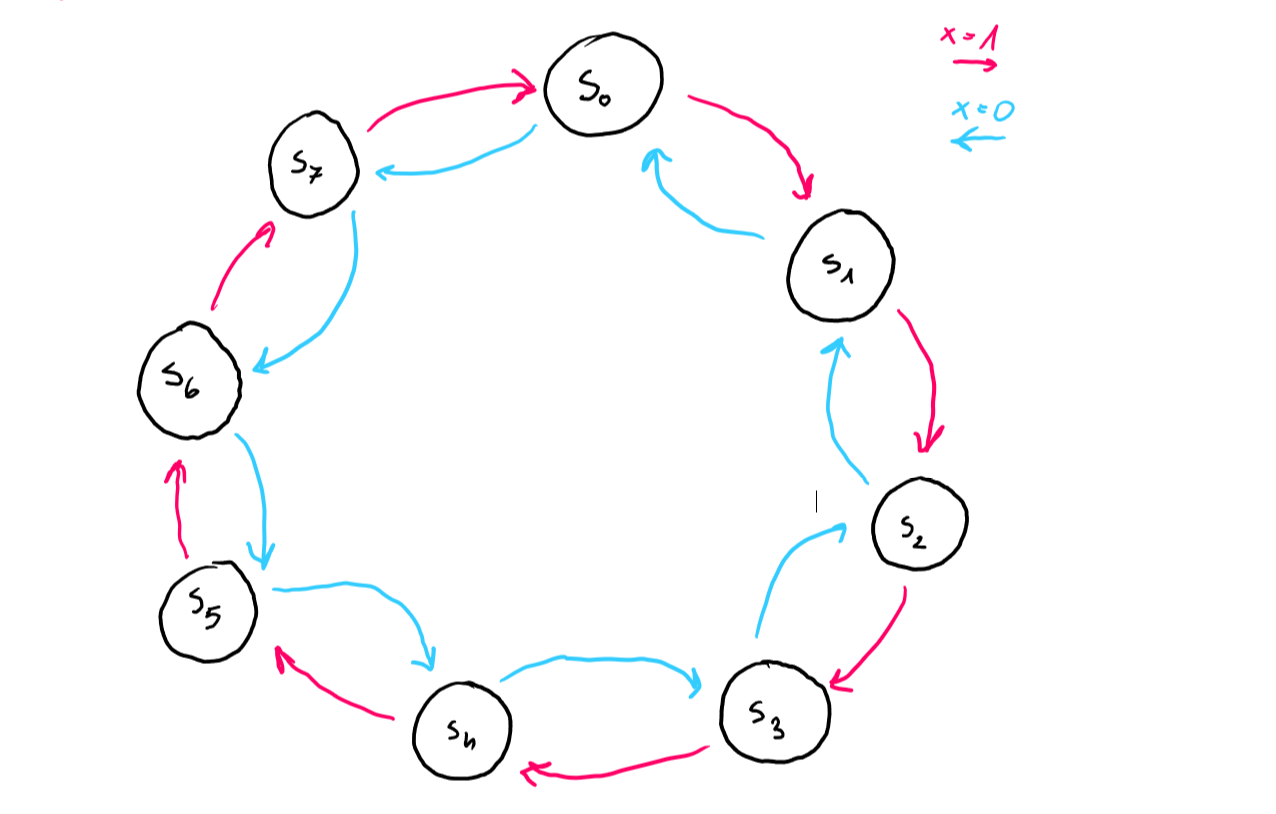
\includegraphics[width=1\textwidth]{szkic.png}
	\caption{Schemat funkcji ("S" z indeksem oznaczają kolejne stany.)}
\end{figure}
Realizujemy funkcję w Logisimie:
\begin{figure}[H]
	\centering
	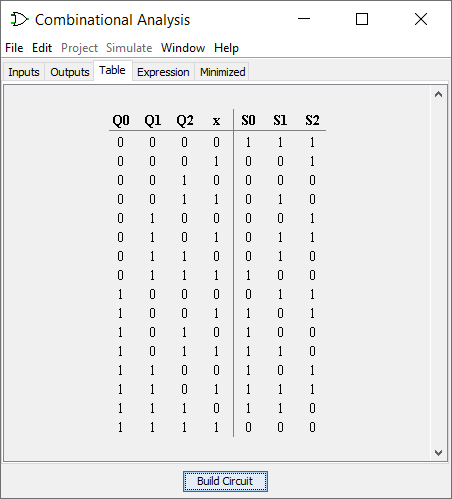
\includegraphics[width=1\textwidth]{tablicaprawdy.png}
	\caption{Tablica prawdy funkcji.}
\end{figure}
Wejście: $Q_0, Q_1, Q_2$ to numer aktualnego stanu zapisany binarnie; x decyduje o kierunku animacji.
Wyjście: $S_0, S_1, S_2$ to numer kolejnego stanu zapisany binarnie.
\begin{figure}[H]
	\centering
	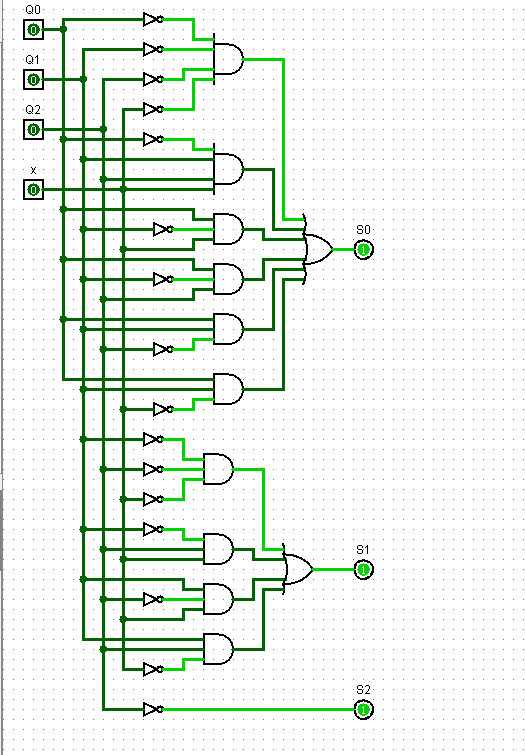
\includegraphics[width=1\textwidth]{realizacja.png}
	\caption{Widok funkcji w Logisimie.}
\end{figure}
\newpage
Testy funkcji dla x=0:
\newline
\begin{minipage}{0.5\textwidth}
\begin{figure}[H]
	\centering
	\includegraphics[width=1\textwidth]{test0_0.png}
\end{figure}
\end{minipage}
\begin{minipage}{0.5\textwidth}
\begin{figure}[H]
	\centering
	\includegraphics[width=1\textwidth]{test0_1.png}
\end{figure}
\end{minipage}
\begin{minipage}{0.5\textwidth}
\begin{figure}[H]
	\centering
	\includegraphics[width=1\textwidth]{test0_2.png}
\end{figure}
\end{minipage}
\begin{minipage}{0.5\textwidth}
\begin{figure}[H]
	\centering
	\includegraphics[width=1\textwidth]{test0_3.png}
\end{figure}
\end{minipage}
\begin{minipage}{0.5\textwidth}
\begin{figure}[H]
	\centering
	\includegraphics[width=1\textwidth]{test0_4.png}
\end{figure}
\end{minipage}
\begin{minipage}{0.5\textwidth}
\begin{figure}[H]
	\centering
	\includegraphics[width=1\textwidth]{test0_5.png}
\end{figure}
\end{minipage}
\begin{minipage}{0.5\textwidth}
\begin{figure}[H]
	\centering
	\includegraphics[width=1\textwidth]{test0_6.png}
\end{figure}
\end{minipage}
\begin{minipage}{0.5\textwidth}
\begin{figure}[H]
	\centering
	\includegraphics[width=1\textwidth]{test0_7.png}
\end{figure}
\end{minipage}
\newpage
Testy funkcji dla x=1:
\newline
\begin{minipage}{0.5\textwidth}
\begin{figure}[H]
	\centering
	\includegraphics[width=1\textwidth]{test1_0.png}
\end{figure}
\end{minipage}
\begin{minipage}{0.5\textwidth}
\begin{figure}[H]
	\centering
	\includegraphics[width=1\textwidth]{test1_1.png}
\end{figure}
\end{minipage}
\begin{minipage}{0.5\textwidth}
\begin{figure}[H]
	\centering
	\includegraphics[width=1\textwidth]{test1_2.png}
\end{figure}
\end{minipage}
\begin{minipage}{0.5\textwidth}
\begin{figure}[H]
	\centering
	\includegraphics[width=1\textwidth]{test1_3.png}
\end{figure}
\end{minipage}
\begin{minipage}{0.5\textwidth}
\begin{figure}[H]
	\centering
	\includegraphics[width=1\textwidth]{test1_4.png}
\end{figure}
\end{minipage}
\begin{minipage}{0.5\textwidth}
\begin{figure}[H]
	\centering
	\includegraphics[width=1\textwidth]{test1_5.png}
\end{figure}
\end{minipage}
\begin{minipage}{0.5\textwidth}
\begin{figure}[H]
	\centering
	\includegraphics[width=1\textwidth]{test1_6.png}
\end{figure}
\end{minipage}
\begin{minipage}{0.5\textwidth}
\begin{figure}[H]
	\centering
	\includegraphics[width=1\textwidth]{test1_7.png}
\end{figure}
\end{minipage}
\begin{center}
\textbf{Wszystkie testy przebiegły pomyślnie.}
\end{center}
\section{Funkcje zmieniające numer stanu na litery}
\subsection{Wyświetlacz 1 (od lewej)}

\begin{figure}[H]
	\centering
	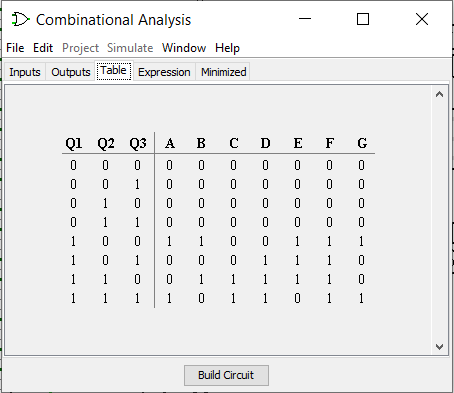
\includegraphics[width=1\textwidth]{JEDEN_Tab.png}
	\caption{Tablica prawdy.}
\end{figure}
\newpage
Stan 000
\begin{figure}[H]
	\centering
	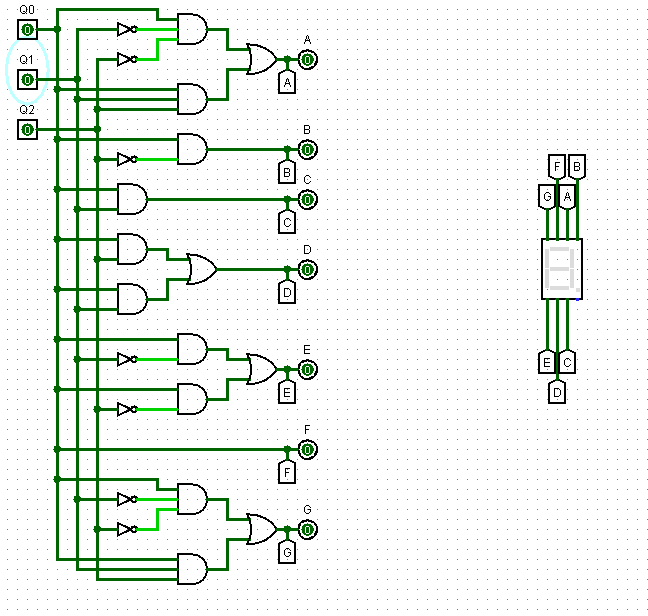
\includegraphics[width=0.7\textwidth]{JEDEN_000.png}
\end{figure}
\newpage
Stan 001
\begin{figure}[H]
	\centering
	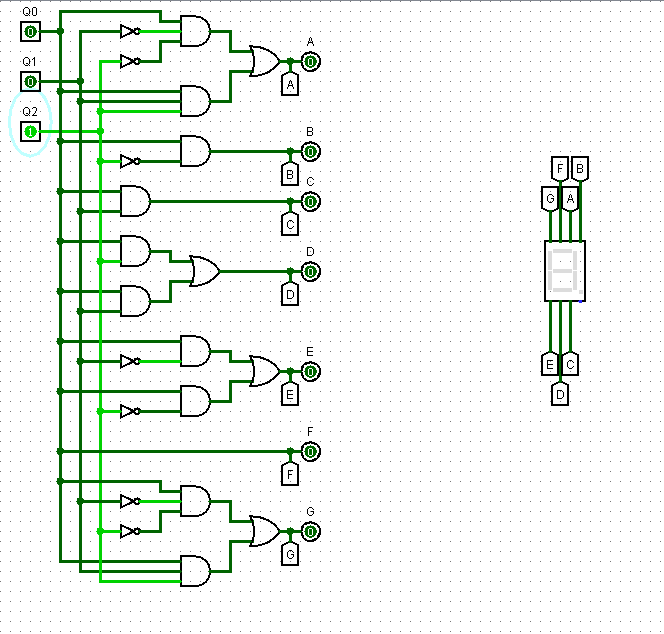
\includegraphics[width=0.7\textwidth]{JEDEN_001.png}
\end{figure}
\newpage
Stan 010
\begin{figure}[H]
	\centering
	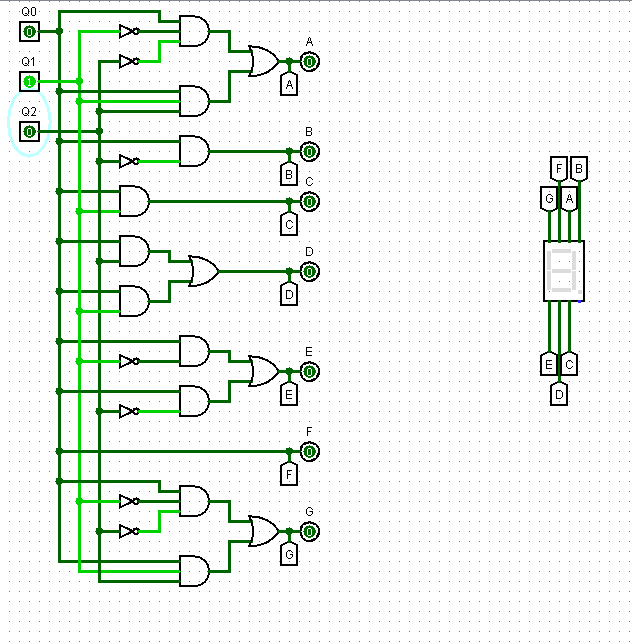
\includegraphics[width=0.7\textwidth]{JEDEN_010.png}
\end{figure}
\newpage
Stan 011
\begin{figure}[H]
	\centering
	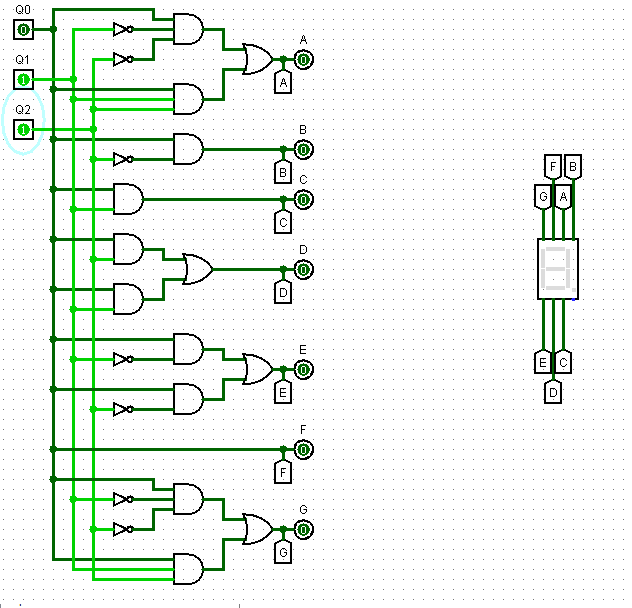
\includegraphics[width=0.7\textwidth]{JEDEN_011.png}
\end{figure}
\newpage
Stan 100
\begin{figure}[H]
	\centering
	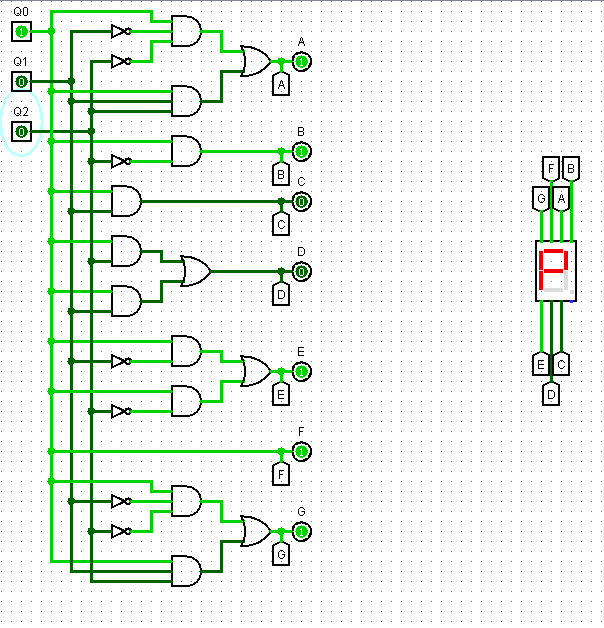
\includegraphics[width=0.7\textwidth]{JEDEN_100.png}
\end{figure}
\newpage
Stan 101
\begin{figure}[H]
	\centering
	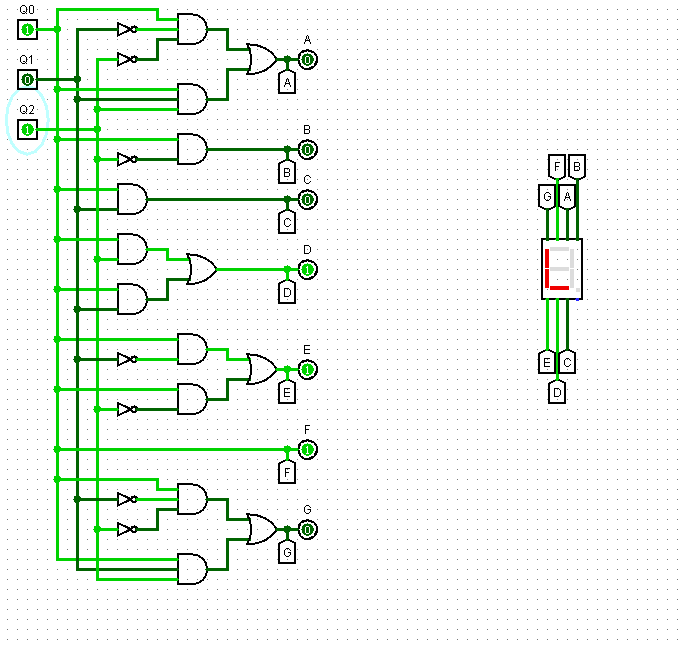
\includegraphics[width=0.7\textwidth]{JEDEN_101.png}
\end{figure}
\newpage
Stan 110
\begin{figure}[H]
	\centering
	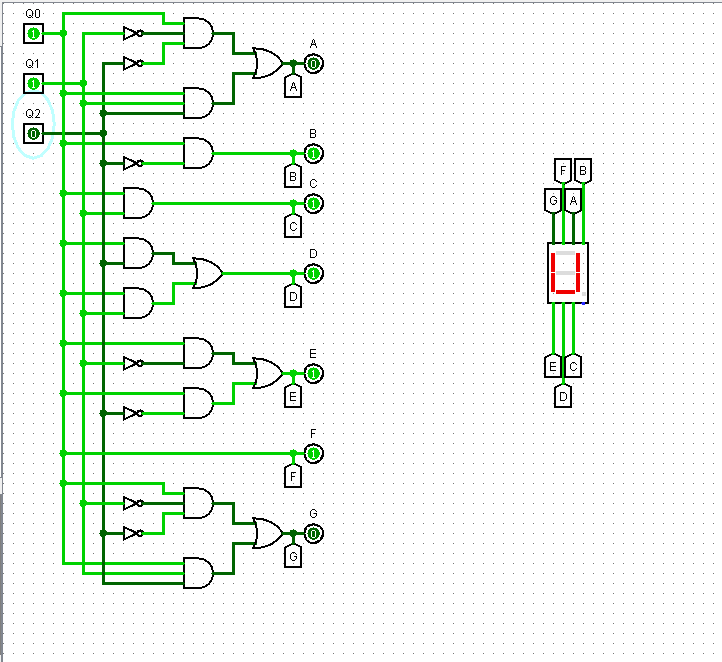
\includegraphics[width=0.7\textwidth]{JEDEN_110.png}
\end{figure}
\newpage
Stan 111
\begin{figure}[H]
	\centering
	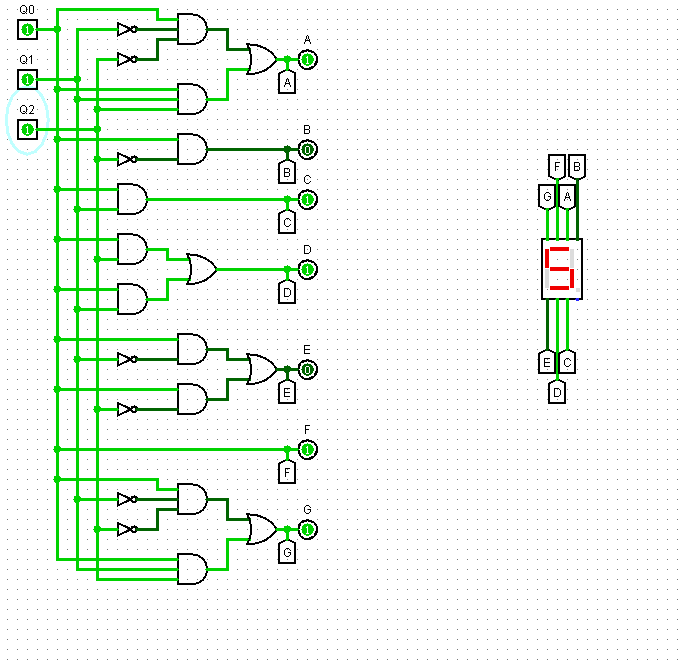
\includegraphics[width=0.7\textwidth]{JEDEN_111.png}
\end{figure}

\subsection{Wyświetlacz 2}
\begin{figure}[H]
	\centering
	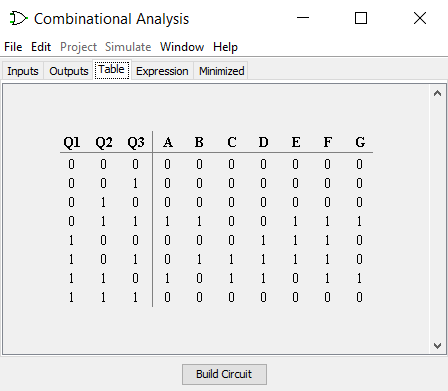
\includegraphics[width=1\textwidth]{DWA_Tab.png}
	\caption{Tablica prawdy.}
\end{figure}
\newpage
Stan 000
\begin{figure}[H]
	\centering
	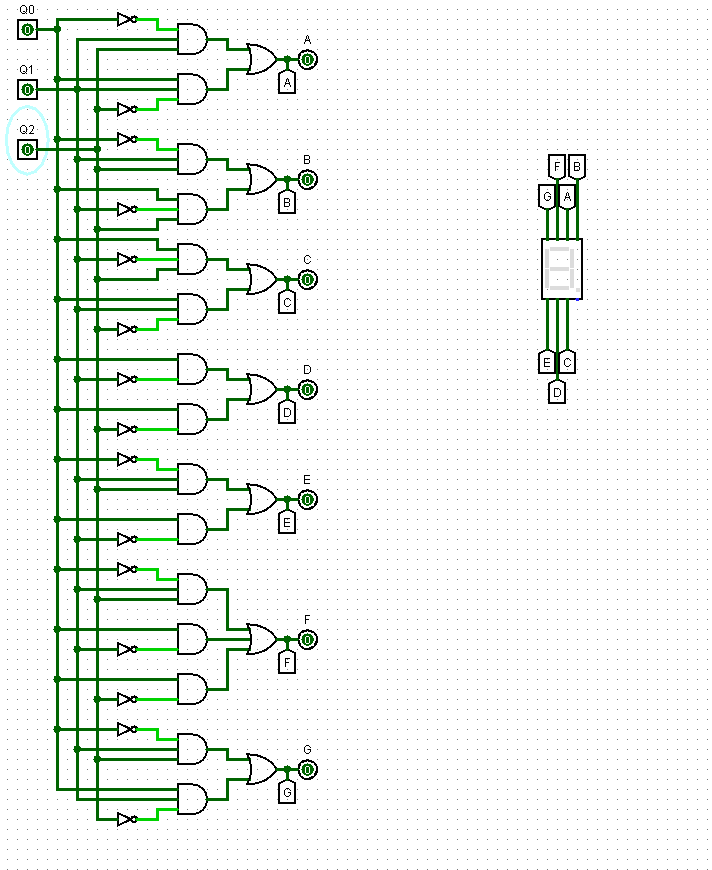
\includegraphics[width=0.7\textwidth]{DWA_000.png}
\end{figure}
\newpage
Stan 001
\begin{figure}[H]
	\centering
	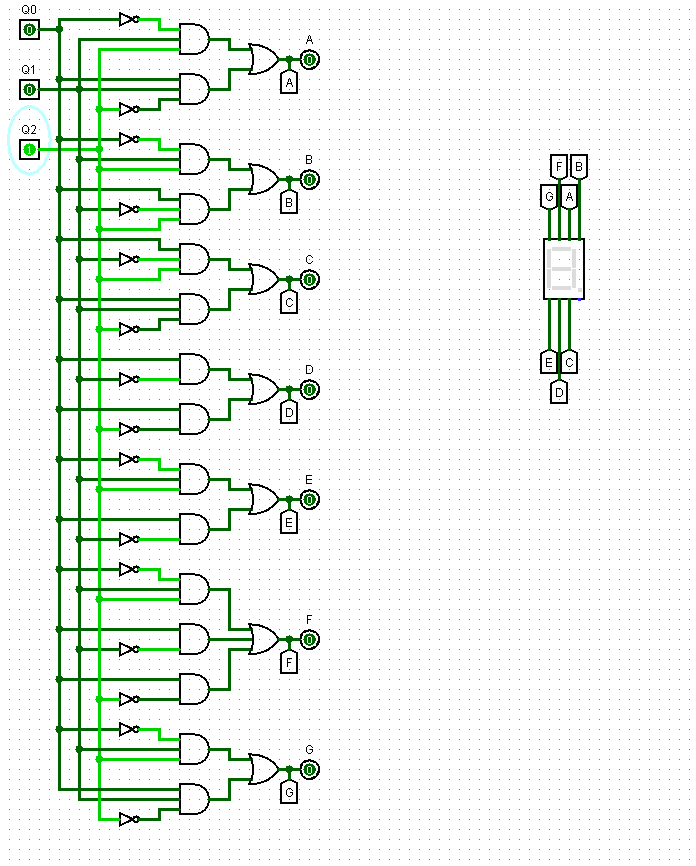
\includegraphics[width=0.7\textwidth]{DWA_001.png}
\end{figure}
\newpage
Stan 010
\begin{figure}[H]
	\centering
	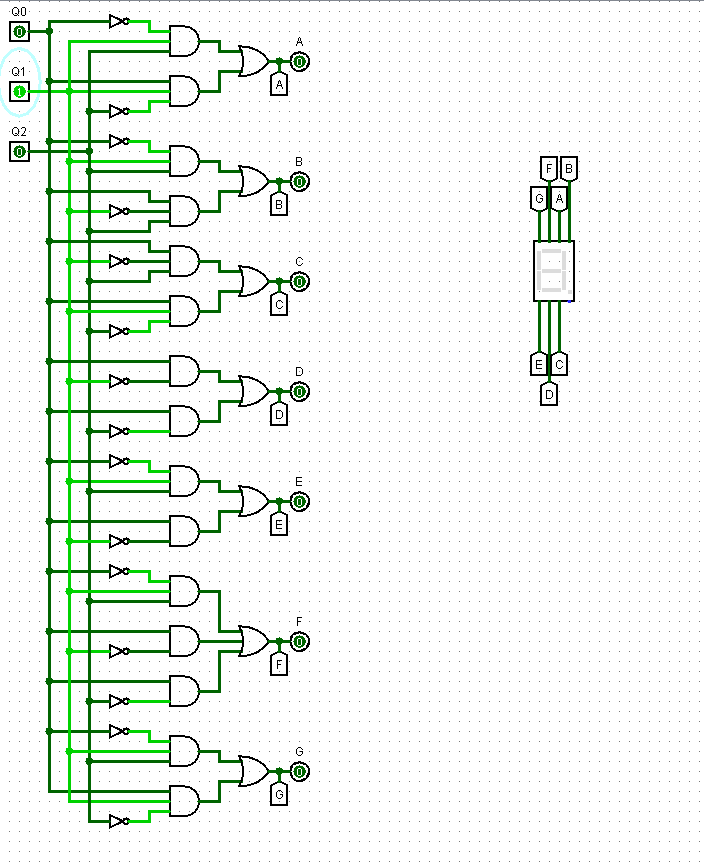
\includegraphics[width=0.7\textwidth]{DWA_010.png}
\end{figure}
\newpage
Stan 011
\begin{figure}[H]
	\centering
	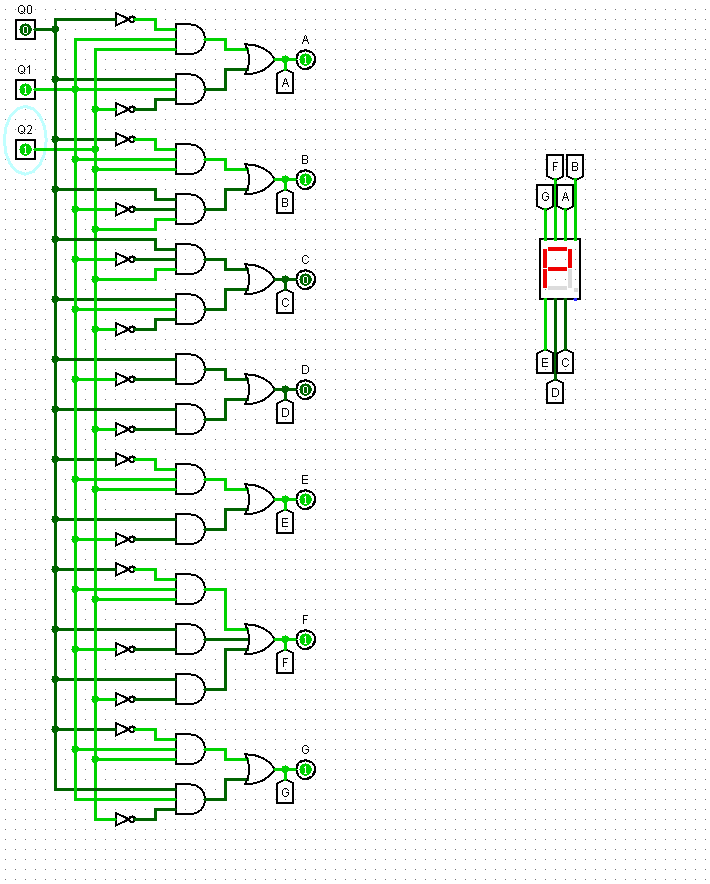
\includegraphics[width=0.7\textwidth]{DWA_011.png}
\end{figure}
\newpage
Stan 100
\begin{figure}[H]
	\centering
	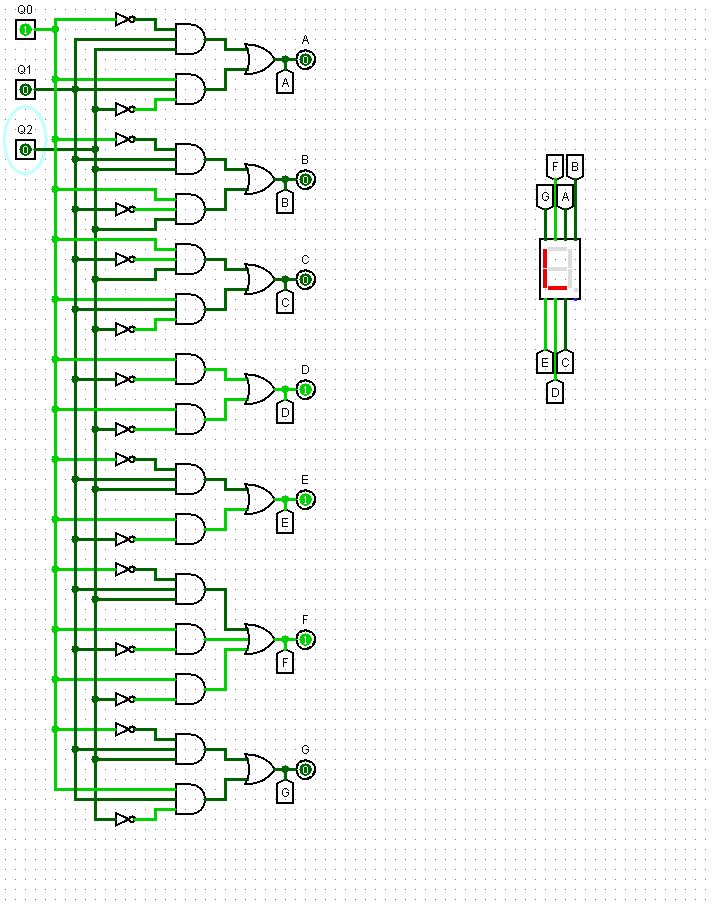
\includegraphics[width=0.7\textwidth]{DWA_100.png}
\end{figure}
\newpage
Stan 101
\begin{figure}[H]
	\centering
	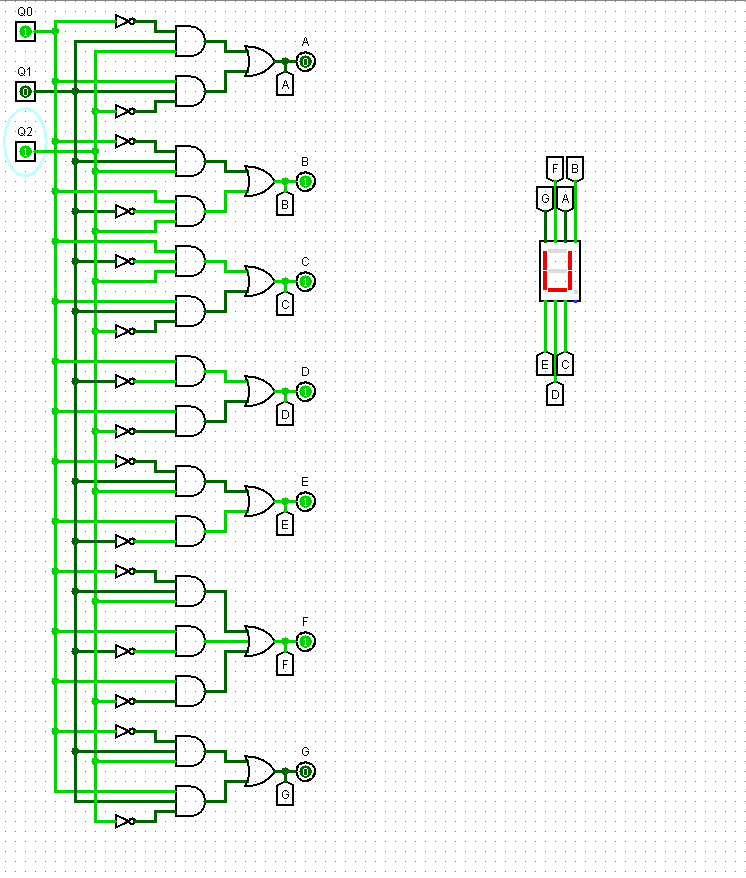
\includegraphics[width=0.7\textwidth]{DWA_101.png}
\end{figure}
\newpage
Stan 110
\begin{figure}[H]
	\centering
	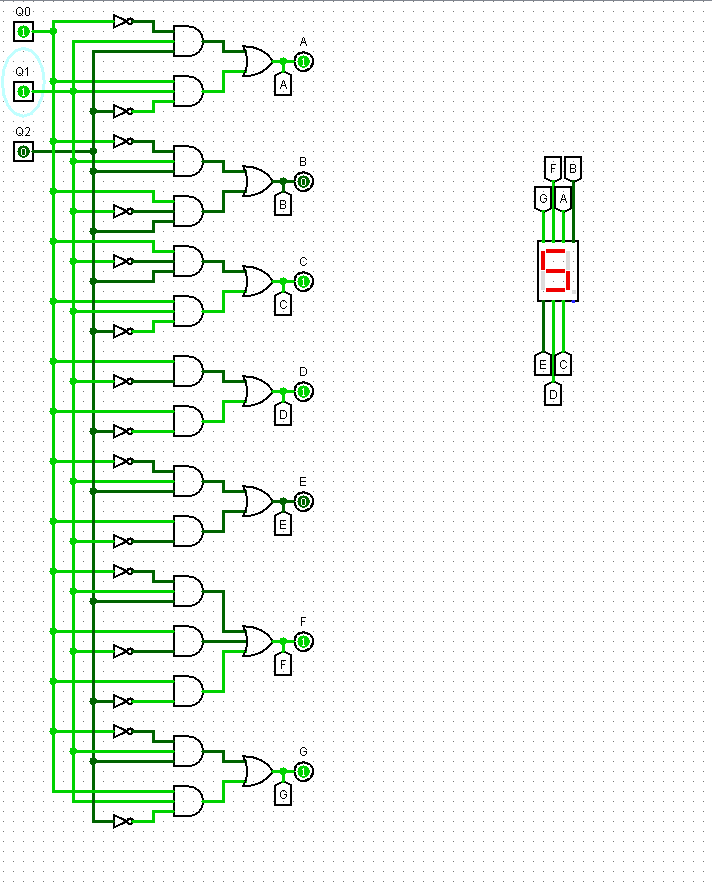
\includegraphics[width=0.7\textwidth]{DWA_110.png}
\end{figure}
\newpage
Stan 111
\begin{figure}[H]
	\centering
	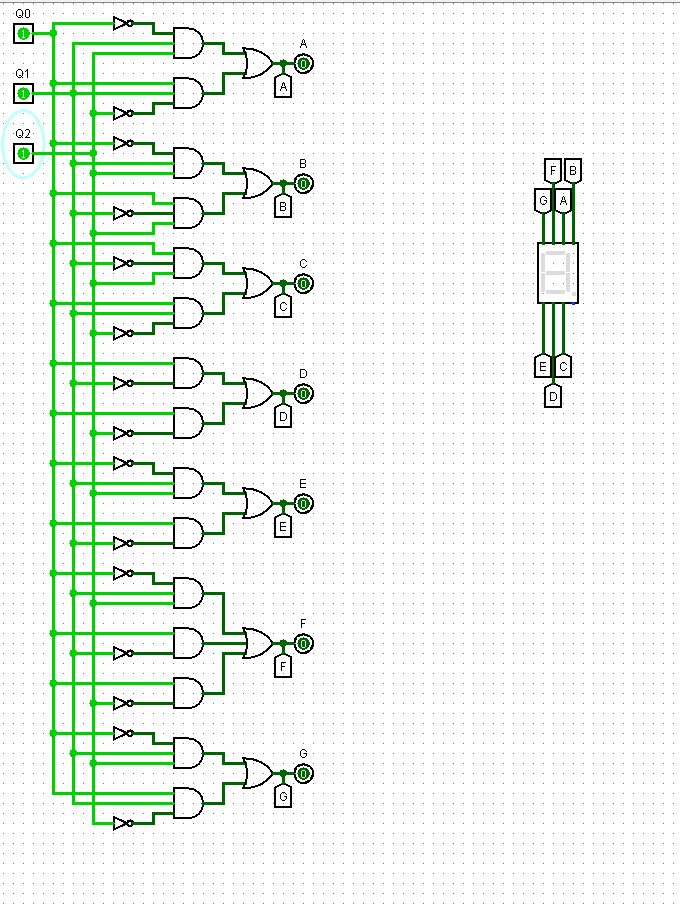
\includegraphics[width=0.7\textwidth]{DWA_111.png}
\end{figure}
\subsection{Wyświetlacz 3}
\begin{figure}[H]
	\centering
	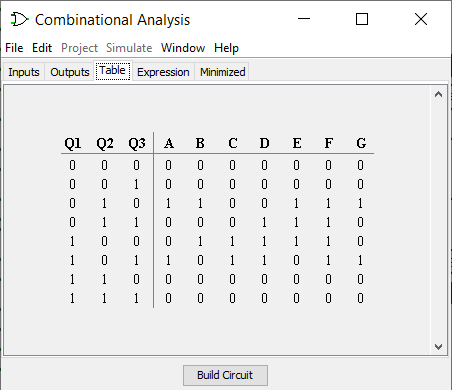
\includegraphics[width=1\textwidth]{TRZY_Tab.png}
	\caption{Tablica prawdy.}
\end{figure}
\newpage
Stan 000
\begin{figure}[H]
	\centering
	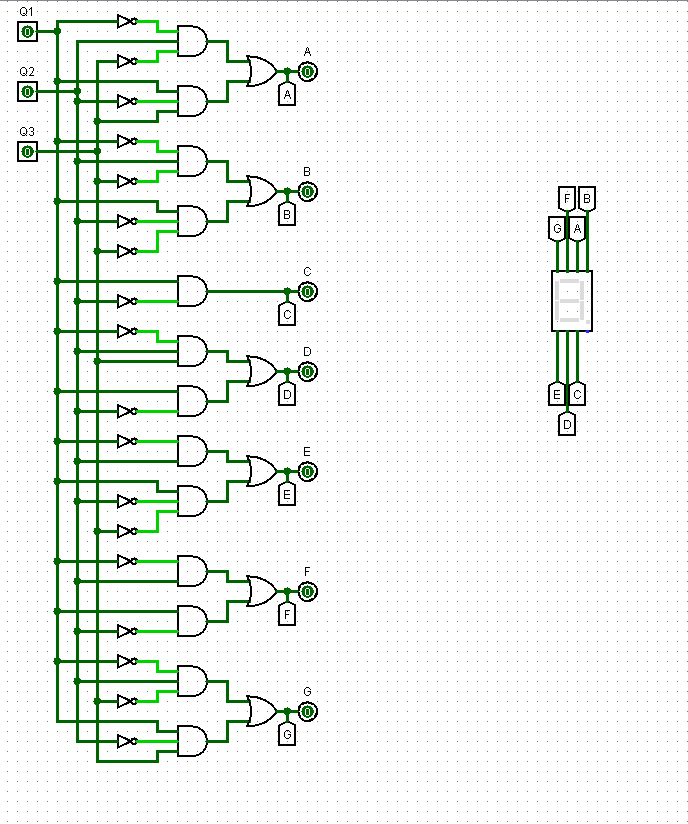
\includegraphics[width=0.7\textwidth]{TTRZY_000.png}
\end{figure}
\newpage
Stan 001
\begin{figure}[H]
	\centering
	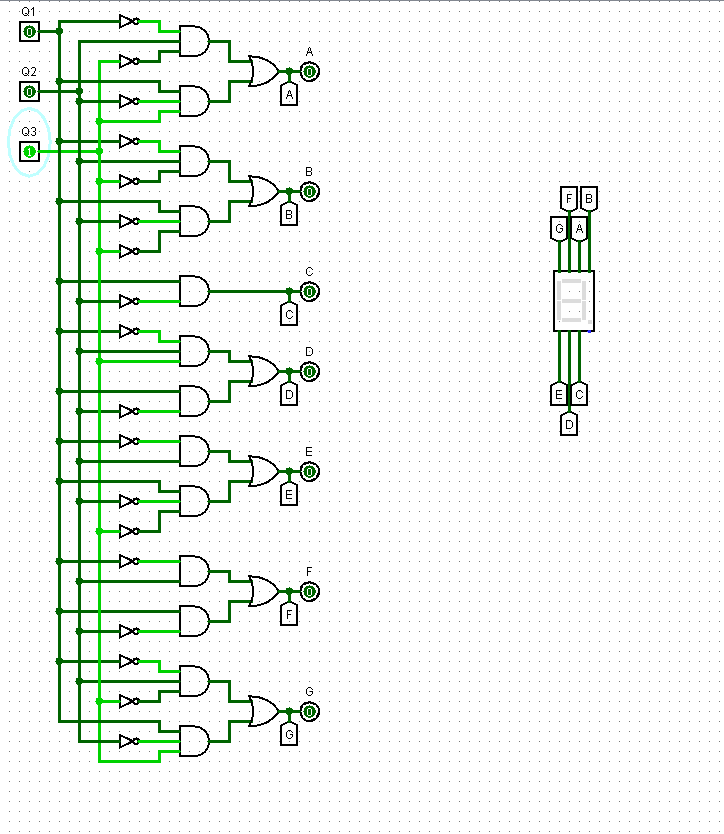
\includegraphics[width=0.7\textwidth]{TTRZY_001.png}
\end{figure}
\newpage
Stan 010
\begin{figure}[H]
	\centering
	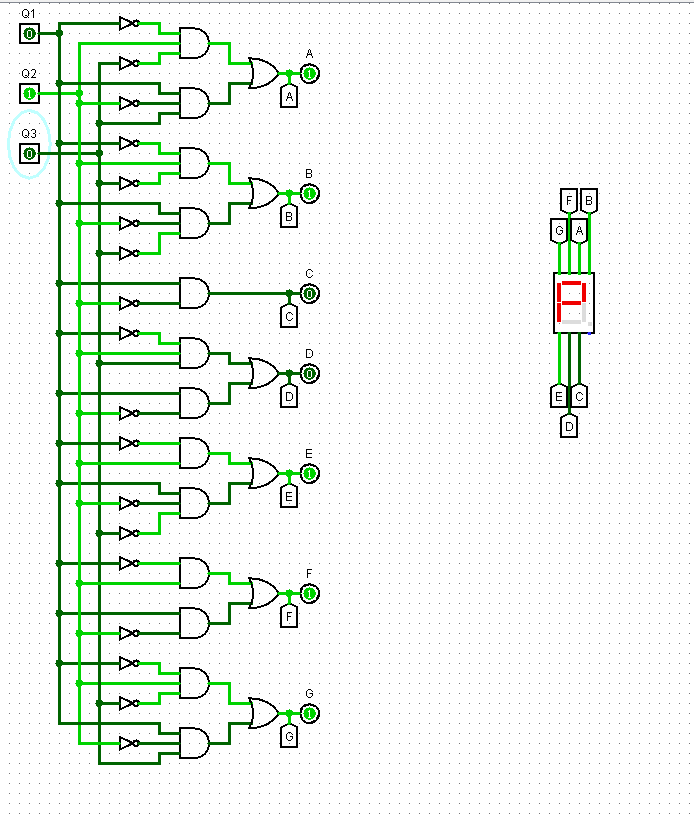
\includegraphics[width=0.7\textwidth]{TTRZY_010.png}
\end{figure}
\newpage
Stan 011
\begin{figure}[H]
	\centering
	\includegraphics[width=0.7\textwidth]{TTRZY_011.png}
\end{figure}
\newpage
Stan 100
\begin{figure}[H]
	\centering
	\includegraphics[width=0.7\textwidth]{TTRZY_100.png}
\end{figure}
\newpage
Stan 101
\begin{figure}[H]
	\centering
	\includegraphics[width=0.7\textwidth]{TTRZY_101.png}
\end{figure}
\newpage
Stan 110
\begin{figure}[H]
	\centering
	\includegraphics[width=0.7\textwidth]{TTRZY_110.png}
\end{figure}
\newpage
Stan 111
\begin{figure}[H]
	\centering
	\includegraphics[width=0.7\textwidth]{TTRZY_111.png}
\end{figure}
\subsection{Wyświetlacz 4}
\begin{figure}[H]
	\centering
	\includegraphics[width=1\textwidth]{CZTERY_Tab.png}
	\caption{Tablica prawdy.}
\end{figure}
\newpage
Stan 000
\begin{figure}[H]
	\centering
	\includegraphics[width=0.7\textwidth]{CZTERY_000.png}
\end{figure}
\newpage
Stan 001	
\begin{figure}[H]
	\centering
	\includegraphics[width=0.7\textwidth]{CZTERY_001.png}
\end{figure}
\newpage
Stan 010
\begin{figure}[H]
	\centering
	\includegraphics[width=0.7\textwidth]{CZTERY_010.png}
\end{figure}
\newpage
Stan 011
\begin{figure}[H]
	\centering
	\includegraphics[width=0.7\textwidth]{CZTERY_011.png}
\end{figure}
\newpage
Stan 100
\begin{figure}[H]
	\centering
	\includegraphics[width=0.7\textwidth]{CZTERY_100.png}
\end{figure}
\newpage
Stan 101
\begin{figure}[H]
	\centering
	\includegraphics[width=0.7\textwidth]{CZTERY_101.png}
\end{figure}
\newpage
Stan 110
\begin{figure}[H]
	\centering
	\includegraphics[width=0.7\textwidth]{CZTERY_110.png}
\end{figure}
\newpage
Stan 111
\begin{figure}[H]
	\centering
	\includegraphics[width=0.7\textwidth]{CZTERY_111.png}
\end{figure}
\section{Przerzutniki}
Dodajemy sygnał zegarowy:
\begin{figure}[H]
	\centering
	\includegraphics[width=0.9\textwidth]{zegar.png}
\end{figure}
\newpage
Dodajemy  sygnał resetu:
\begin{figure}[H]
	\centering
	\includegraphics[width=0.7\textwidth]{reset.png}
\end{figure}
Dodajemy cztery wyświetlacze 7-segmentowe połączone z odpowiednimi funkcjami zmieniającymi numer stanu na litery i przeprowadzamy testy.
\newpage
\section{Testy}
Stan 0
\begin{figure}[H]
	\centering
	\includegraphics[width=1.25\textwidth]{0.png}
\end{figure}
\newpage
Stan 1
\begin{figure}[H]
	\centering
	\includegraphics[width=1.0\textwidth]{1.png}
\end{figure}
\newpage
Stan 2
\begin{figure}[H]
	\centering
	\includegraphics[width=1.2\textwidth]{2.png}
\end{figure}
\newpage
Stan 3
\begin{figure}[H]
	\centering
	\includegraphics[width=1.2\textwidth]{3.png}
\end{figure}
\newpage
Stan 4
\begin{figure}[H]
	\centering
	\includegraphics[width=1.2\textwidth]{4.png}
\end{figure}
\newpage
Stan 5
\begin{figure}[H]
	\centering
	\includegraphics[width=1.2\textwidth]{5.png}
\end{figure}
\newpage
Stan 6
\begin{figure}[H]
	\centering
	\includegraphics[width=1.2\textwidth]{6.png}
\end{figure}
\newpage
Stan 7
\begin{figure}[H]
	\centering
	\includegraphics[width=1.2\textwidth]{7.png}
\end{figure}
\end{document}
